$y^2=8x^2$ desde $x=1$ a $x=8$.

\nopagebreak
\begin{align*}
y = \pm \sqrt{8} x = \pm 2\sqrt{2} x. \\
\text{Tomamos la rama positiva: } y = 2\sqrt{2} x. \\
y' = 2\sqrt{2}. \\
L &= \int_{1}^{8} \sqrt{1 + (y')^2} \, dx \\
&= \int_{1}^{8} \sqrt{1 + (2\sqrt{2})^2} \, dx \\
&= \int_{1}^{8} \sqrt{1 + 8} \, dx = \int_{1}^{8} 3 \, dx \\
&= 3(8-1) = 21
\end{align*}

\[
\boxed{\displaystyle 21}
\]

\begin{center}
    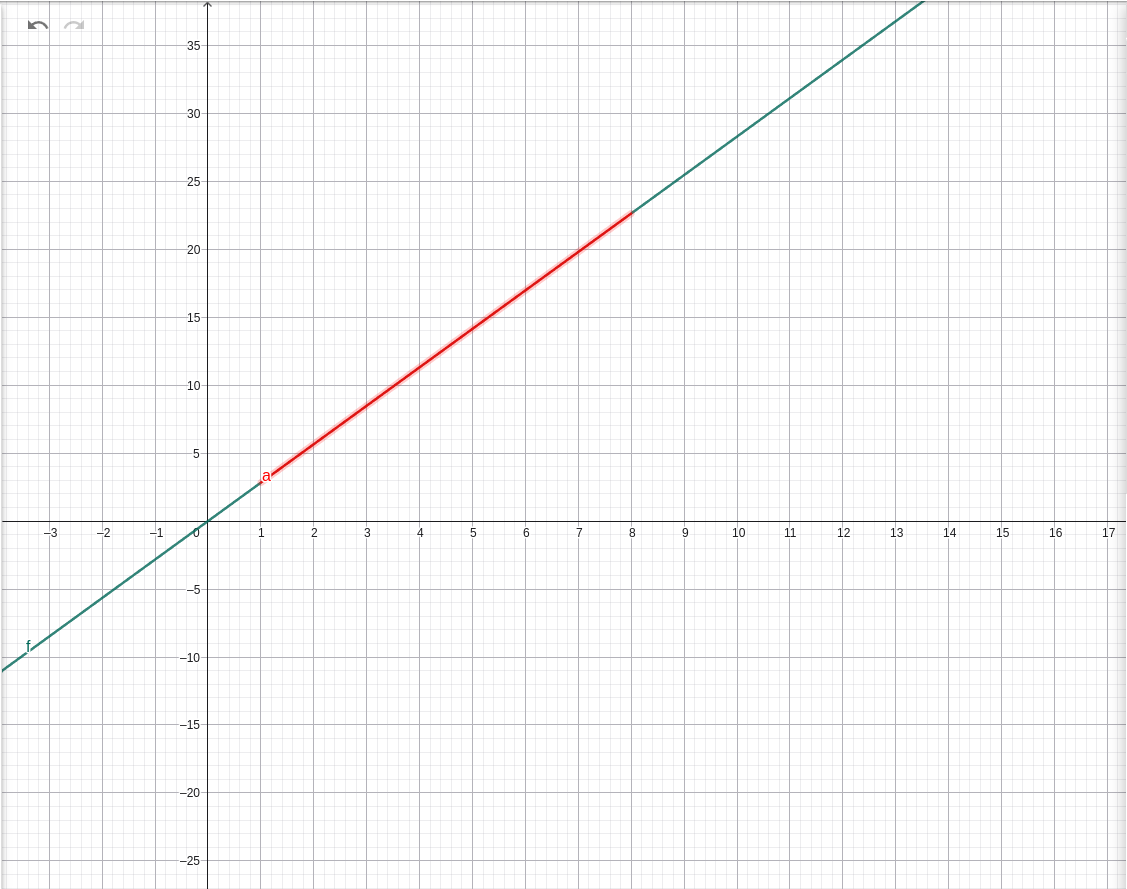
\includegraphics[width=0.5\textwidth]{Graficas/ejer45.png}
\end{center}
